\documentclass[twoside]{book}

% Packages required by doxygen
\usepackage{fixltx2e}
\usepackage{calc}
\usepackage{doxygen}
\usepackage[export]{adjustbox} % also loads graphicx
\usepackage{graphicx}
\usepackage[utf8]{inputenc}
\usepackage{makeidx}
\usepackage{multicol}
\usepackage{multirow}
\PassOptionsToPackage{warn}{textcomp}
\usepackage{textcomp}
\usepackage[nointegrals]{wasysym}
\usepackage[table]{xcolor}

% Font selection
\usepackage[T1]{fontenc}
\usepackage[scaled=.90]{helvet}
\usepackage{courier}
\usepackage{amssymb}
\usepackage{sectsty}
\renewcommand{\familydefault}{\sfdefault}
\allsectionsfont{%
  \fontseries{bc}\selectfont%
  \color{darkgray}%
}
\renewcommand{\DoxyLabelFont}{%
  \fontseries{bc}\selectfont%
  \color{darkgray}%
}
\newcommand{\+}{\discretionary{\mbox{\scriptsize$\hookleftarrow$}}{}{}}

% Page & text layout
\usepackage{geometry}
\geometry{%
  a4paper,%
  top=2.5cm,%
  bottom=2.5cm,%
  left=2.5cm,%
  right=2.5cm%
}
\tolerance=750
\hfuzz=15pt
\hbadness=750
\setlength{\emergencystretch}{15pt}
\setlength{\parindent}{0cm}
\setlength{\parskip}{3ex plus 2ex minus 2ex}
\makeatletter
\renewcommand{\paragraph}{%
  \@startsection{paragraph}{4}{0ex}{-1.0ex}{1.0ex}{%
    \normalfont\normalsize\bfseries\SS@parafont%
  }%
}
\renewcommand{\subparagraph}{%
  \@startsection{subparagraph}{5}{0ex}{-1.0ex}{1.0ex}{%
    \normalfont\normalsize\bfseries\SS@subparafont%
  }%
}
\makeatother

% Headers & footers
\usepackage{fancyhdr}
\pagestyle{fancyplain}
\fancyhead[LE]{\fancyplain{}{\bfseries\thepage}}
\fancyhead[CE]{\fancyplain{}{}}
\fancyhead[RE]{\fancyplain{}{\bfseries\leftmark}}
\fancyhead[LO]{\fancyplain{}{\bfseries\rightmark}}
\fancyhead[CO]{\fancyplain{}{}}
\fancyhead[RO]{\fancyplain{}{\bfseries\thepage}}
\fancyfoot[LE]{\fancyplain{}{}}
\fancyfoot[CE]{\fancyplain{}{}}
\fancyfoot[RE]{\fancyplain{}{\bfseries\scriptsize Generated by Doxygen }}
\fancyfoot[LO]{\fancyplain{}{\bfseries\scriptsize Generated by Doxygen }}
\fancyfoot[CO]{\fancyplain{}{}}
\fancyfoot[RO]{\fancyplain{}{}}
\renewcommand{\footrulewidth}{0.4pt}
\renewcommand{\chaptermark}[1]{%
  \markboth{#1}{}%
}
\renewcommand{\sectionmark}[1]{%
  \markright{\thesection\ #1}%
}

% Indices & bibliography
\usepackage{natbib}
\usepackage[titles]{tocloft}
\setcounter{tocdepth}{3}
\setcounter{secnumdepth}{5}
\makeindex

% Hyperlinks (required, but should be loaded last)
\usepackage{ifpdf}
\ifpdf
  \usepackage[pdftex,pagebackref=true]{hyperref}
\else
  \usepackage[ps2pdf,pagebackref=true]{hyperref}
\fi
\hypersetup{%
  colorlinks=true,%
  linkcolor=blue,%
  citecolor=blue,%
  unicode%
}

% Custom commands
\newcommand{\clearemptydoublepage}{%
  \newpage{\pagestyle{empty}\cleardoublepage}%
}

\usepackage{caption}
\captionsetup{labelsep=space,justification=centering,font={bf},singlelinecheck=off,skip=4pt,position=top}

%===== C O N T E N T S =====

\begin{document}

% Titlepage & ToC
\hypersetup{pageanchor=false,
             bookmarksnumbered=true,
             pdfencoding=unicode
            }
\pagenumbering{alph}
\begin{titlepage}
\vspace*{7cm}
\begin{center}%
{\Large H\+T\+TP server \\[1ex]\large 1.\+2 }\\
\vspace*{1cm}
{\large Generated by Doxygen 1.8.13}\\
\end{center}
\end{titlepage}
\clearemptydoublepage
\pagenumbering{roman}
\tableofcontents
\clearemptydoublepage
\pagenumbering{arabic}
\hypersetup{pageanchor=true}

%--- Begin generated contents ---
\chapter{Hierarchical Index}
\section{Class Hierarchy}
This inheritance list is sorted roughly, but not completely, alphabetically\+:\begin{DoxyCompactList}
\item condition\+\_\+variable\begin{DoxyCompactList}
\item \contentsline{section}{cond\+\_\+var}{\pageref{classcond__var}}{}
\end{DoxyCompactList}
\item \contentsline{section}{page}{\pageref{classpage}}{}
\item \contentsline{section}{paragraph}{\pageref{classparagraph}}{}
\item \contentsline{section}{server}{\pageref{classserver}}{}
\item \contentsline{section}{server\+\_\+manager}{\pageref{classserver__manager}}{}
\item \contentsline{section}{session}{\pageref{classsession}}{}
\end{DoxyCompactList}

\chapter{Class Index}
\section{Class List}
Here are the classes, structs, unions and interfaces with brief descriptions\+:\begin{DoxyCompactList}
\item\contentsline{section}{\hyperlink{classcond__var}{cond\+\_\+var} \\*Condition variables are used for communication between threads }{\pageref{classcond__var}}{}
\item\contentsline{section}{\hyperlink{classpage}{page} \\*Page class contains array of paragraphs and function to work with them }{\pageref{classpage}}{}
\item\contentsline{section}{\hyperlink{classparagraph}{paragraph} \\*Paragraph class to contain paragraphs of the text }{\pageref{classparagraph}}{}
\item\contentsline{section}{\hyperlink{classserver}{server} \\*H\+T\+TP server\textquotesingle{}s main class }{\pageref{classserver}}{}
\item\contentsline{section}{\hyperlink{classserver__manager}{server\+\_\+manager} }{\pageref{classserver__manager}}{}
\item\contentsline{section}{\hyperlink{classsession}{session} \\*Operates with requests and sends the respond }{\pageref{classsession}}{}
\end{DoxyCompactList}

\chapter{File Index}
\section{File List}
Here is a list of all documented files with brief descriptions\+:\begin{DoxyCompactList}
\item\contentsline{section}{\hyperlink{_servers_8h}{Servers.\+h} \\*H\+T\+TP server with support of G\+ET, H\+E\+AD, P\+O\+ST requests }{\pageref{_servers_8h}}{}
\end{DoxyCompactList}

\chapter{Class Documentation}
\hypertarget{classcond__var}{}\section{cond\+\_\+var Class Reference}
\label{classcond__var}\index{cond\+\_\+var@{cond\+\_\+var}}


condition variables are used for communication between threads  




{\ttfamily \#include $<$Servers.\+h$>$}

Inheritance diagram for cond\+\_\+var\+:\begin{figure}[H]
\begin{center}
\leavevmode
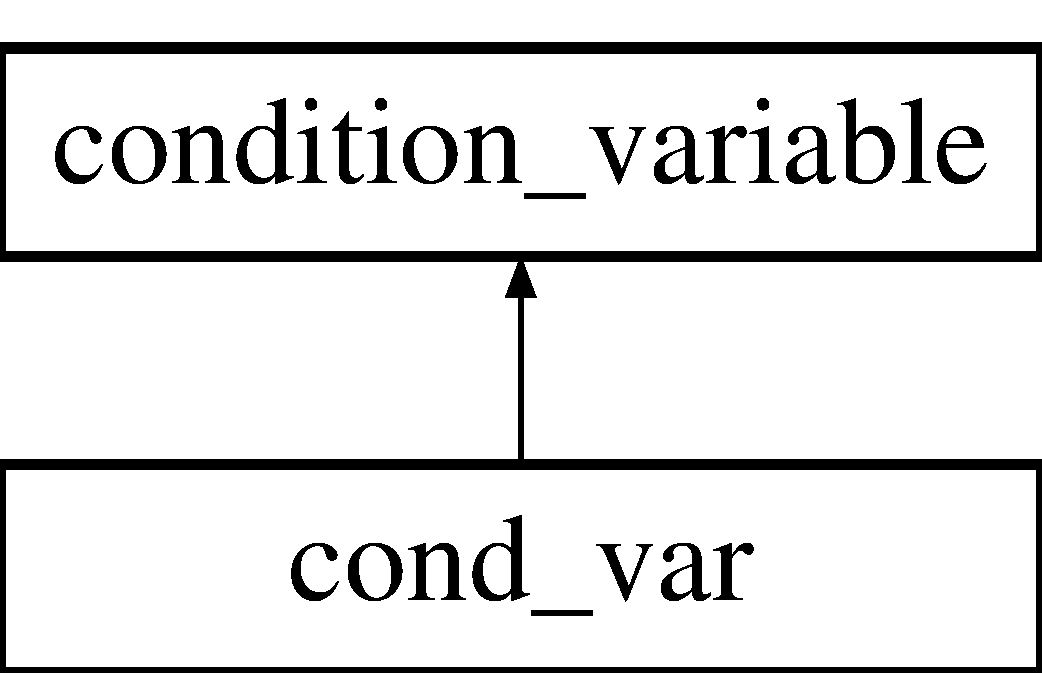
\includegraphics[height=2.000000cm]{classcond__var}
\end{center}
\end{figure}
\subsection*{Public Member Functions}
\begin{DoxyCompactItemize}
\item 
\mbox{\Hypertarget{classcond__var_a93dbd1d43db5b2c64fd740c240e2418c}\label{classcond__var_a93dbd1d43db5b2c64fd740c240e2418c}} 
\hyperlink{classcond__var_a93dbd1d43db5b2c64fd740c240e2418c}{cond\+\_\+var} ()
\begin{DoxyCompactList}\small\item\em standard constructor \end{DoxyCompactList}\item 
\mbox{\Hypertarget{classcond__var_aeee90ce194ac52729ec961359d489bfb}\label{classcond__var_aeee90ce194ac52729ec961359d489bfb}} 
\hyperlink{classcond__var_aeee90ce194ac52729ec961359d489bfb}{$\sim$cond\+\_\+var} ()
\begin{DoxyCompactList}\small\item\em standard destructor, no extra memory is used \end{DoxyCompactList}\item 
\mbox{\Hypertarget{classcond__var_a41eff0f79f6695bbaca67153559c4885}\label{classcond__var_a41eff0f79f6695bbaca67153559c4885}} 
void \hyperlink{classcond__var_a41eff0f79f6695bbaca67153559c4885}{set\+\_\+data} (boost\+::asio\+::io\+\_\+context \&iocont, \hyperlink{classserver}{server} $\ast$serv, \hyperlink{classsession}{session} $\ast$s)
\begin{DoxyCompactList}\small\item\em initializes the values of this class\textquotesingle{} object\textquotesingle{}s members \end{DoxyCompactList}\item 
\mbox{\Hypertarget{classcond__var_aa517d0951844aaa609600903635b887d}\label{classcond__var_aa517d0951844aaa609600903635b887d}} 
boost\+::asio\+::io\+\_\+context $\ast$ \hyperlink{classcond__var_aa517d0951844aaa609600903635b887d}{get\+\_\+context} ()
\begin{DoxyCompactList}\small\item\em returns the current io\+\_\+context \end{DoxyCompactList}\item 
\mbox{\Hypertarget{classcond__var_ae55f3716e292cca887be939fe8f10c26}\label{classcond__var_ae55f3716e292cca887be939fe8f10c26}} 
\hyperlink{classserver}{server} $\ast$ \hyperlink{classcond__var_ae55f3716e292cca887be939fe8f10c26}{get\+\_\+server} ()
\begin{DoxyCompactList}\small\item\em returns the pointer to current server \end{DoxyCompactList}\item 
\mbox{\Hypertarget{classcond__var_a624ff85e7f2850661ec9c408ef1a7a26}\label{classcond__var_a624ff85e7f2850661ec9c408ef1a7a26}} 
\hyperlink{classsession}{session} $\ast$ \hyperlink{classcond__var_a624ff85e7f2850661ec9c408ef1a7a26}{get\+\_\+session} ()
\begin{DoxyCompactList}\small\item\em returns the pointer to current session \end{DoxyCompactList}\end{DoxyCompactItemize}


\subsection{Detailed Description}
condition variables are used for communication between threads 

The documentation for this class was generated from the following file\+:\begin{DoxyCompactItemize}
\item 
Servers.\+h\end{DoxyCompactItemize}

\hypertarget{classpage}{}\section{page Class Reference}
\label{classpage}\index{page@{page}}


page class contains array of paragraphs and function to work with them  




{\ttfamily \#include $<$Servers.\+h$>$}

\subsection*{Public Member Functions}
\begin{DoxyCompactItemize}
\item 
\mbox{\Hypertarget{classpage_ab0cfd233d0d3381cf9a7b83e0fddc9ee}\label{classpage_ab0cfd233d0d3381cf9a7b83e0fddc9ee}} 
\hyperlink{classpage_ab0cfd233d0d3381cf9a7b83e0fddc9ee}{page} ()
\begin{DoxyCompactList}\small\item\em default constructor that puts 0\textquotesingle{}s to member fields \end{DoxyCompactList}\item 
\hyperlink{classpage_a70d21de949a1787fb6db224844b8dce9}{page} (char $\ast$pname)
\item 
\mbox{\Hypertarget{classpage_a599995602a1df90cd29b26dd955cd93e}\label{classpage_a599995602a1df90cd29b26dd955cd93e}} 
\hyperlink{classpage_a599995602a1df90cd29b26dd955cd93e}{$\sim$page} ()
\begin{DoxyCompactList}\small\item\em destructor that calls del\+\_\+page \end{DoxyCompactList}\item 
\mbox{\Hypertarget{classpage_aa54645bcbff5f2747b65a3eb4bb09b7c}\label{classpage_aa54645bcbff5f2747b65a3eb4bb09b7c}} 
char $\ast$ \hyperlink{classpage_aa54645bcbff5f2747b65a3eb4bb09b7c}{get\+\_\+page\+\_\+name} ()
\begin{DoxyCompactList}\small\item\em returns current page name \end{DoxyCompactList}\item 
\mbox{\Hypertarget{classpage_ad9532e48c5e2359694625de13e3825c1}\label{classpage_ad9532e48c5e2359694625de13e3825c1}} 
bool \hyperlink{classpage_ad9532e48c5e2359694625de13e3825c1}{is\+\_\+page} (char $\ast$name)
\begin{DoxyCompactList}\small\item\em compares current page name with name \end{DoxyCompactList}\item 
int \hyperlink{classpage_a5eae57fad910ef40d723c1808eeabad9}{open\+\_\+page} (char $\ast$pname)
\item 
\mbox{\Hypertarget{classpage_ad3851ad84faf2677e8a50087e0627509}\label{classpage_ad3851ad84faf2677e8a50087e0627509}} 
int \hyperlink{classpage_ad3851ad84faf2677e8a50087e0627509}{delete\+\_\+page} ()
\begin{DoxyCompactList}\small\item\em deletes current page, returns 0 if OK, 1 if not \end{DoxyCompactList}\item 
int \hyperlink{classpage_a1c55a90abfcc823c8216c9dad7660f24}{del\+\_\+paragraph} (int num)
\item 
int \hyperlink{classpage_a03e597adceb2d5147a1729d6517df5b4}{add\+\_\+to\+\_\+par} (int num, char $\ast$text)
\item 
\mbox{\Hypertarget{classpage_a5182baae92ba16e0d8ac1c1b97cda5c0}\label{classpage_a5182baae92ba16e0d8ac1c1b97cda5c0}} 
int \hyperlink{classpage_a5182baae92ba16e0d8ac1c1b97cda5c0}{insert\+\_\+paragraph\+\_\+at\+\_\+end} (char $\ast$text)
\begin{DoxyCompactList}\small\item\em adds new paragraph at the end of the array, returns length of text if OK, -\/1 if not \end{DoxyCompactList}\item 
\mbox{\Hypertarget{classpage_a5cbc74c74b3b2296bc76fe5496cff59f}\label{classpage_a5cbc74c74b3b2296bc76fe5496cff59f}} 
int \hyperlink{classpage_a5cbc74c74b3b2296bc76fe5496cff59f}{write\+\_\+page} ()
\begin{DoxyCompactList}\small\item\em writes changes of the page on the disk, returns 0 if OK, 1 if not \end{DoxyCompactList}\end{DoxyCompactItemize}
\subsection*{Static Public Member Functions}
\begin{DoxyCompactItemize}
\item 
\mbox{\Hypertarget{classpage_a4030e9084e093da1687ed0a0ff34c9d2}\label{classpage_a4030e9084e093da1687ed0a0ff34c9d2}} 
static int \hyperlink{classpage_a4030e9084e093da1687ed0a0ff34c9d2}{delete\+\_\+page} (char $\ast$name)
\begin{DoxyCompactList}\small\item\em deletes page from the drive by its name \end{DoxyCompactList}\end{DoxyCompactItemize}
\subsection*{Protected Member Functions}
\begin{DoxyCompactItemize}
\item 
\mbox{\Hypertarget{classpage_af3155afb8335de30b52d4280f390c398}\label{classpage_af3155afb8335de30b52d4280f390c398}} 
int \hyperlink{classpage_af3155afb8335de30b52d4280f390c398}{open\+\_\+page} ()
\begin{DoxyCompactList}\small\item\em hiden function to open page by the name in pagename \end{DoxyCompactList}\item 
\mbox{\Hypertarget{classpage_acb20752136c88c804d6f3f6ef0569737}\label{classpage_acb20752136c88c804d6f3f6ef0569737}} 
int \hyperlink{classpage_acb20752136c88c804d6f3f6ef0569737}{del\+\_\+page} ()
\begin{DoxyCompactList}\small\item\em hiden function to destroy all allocated memory if any \end{DoxyCompactList}\end{DoxyCompactItemize}
\subsection*{Protected Attributes}
\begin{DoxyCompactItemize}
\item 
\mbox{\Hypertarget{classpage_ac0fc49e219397088606ebdaa04e5728f}\label{classpage_ac0fc49e219397088606ebdaa04e5728f}} 
std\+::array$<$ \hyperlink{classparagraph}{paragraph}, 100 $>$ {\bfseries par\+\_\+arr}
\item 
\mbox{\Hypertarget{classpage_ac98ed4bbad67f1981e117ccc488cc1b7}\label{classpage_ac98ed4bbad67f1981e117ccc488cc1b7}} 
int {\bfseries numpar}
\item 
\mbox{\Hypertarget{classpage_a362475983bb94ce58bb55d49c2646ec9}\label{classpage_a362475983bb94ce58bb55d49c2646ec9}} 
char $\ast$ {\bfseries pagename}
\end{DoxyCompactItemize}


\subsection{Detailed Description}
page class contains array of paragraphs and function to work with them 

\subsection{Constructor \& Destructor Documentation}
\mbox{\Hypertarget{classpage_a70d21de949a1787fb6db224844b8dce9}\label{classpage_a70d21de949a1787fb6db224844b8dce9}} 
\index{page@{page}!page@{page}}
\index{page@{page}!page@{page}}
\subsubsection{\texorpdfstring{page()}{page()}}
{\footnotesize\ttfamily page\+::page (\begin{DoxyParamCaption}\item[{char $\ast$}]{pname }\end{DoxyParamCaption})\hspace{0.3cm}{\ttfamily [inline]}}

constructor pname --- name of the page to open and process stores pname in pagename, also opens this page 

\subsection{Member Function Documentation}
\mbox{\Hypertarget{classpage_a03e597adceb2d5147a1729d6517df5b4}\label{classpage_a03e597adceb2d5147a1729d6517df5b4}} 
\index{page@{page}!add\+\_\+to\+\_\+par@{add\+\_\+to\+\_\+par}}
\index{add\+\_\+to\+\_\+par@{add\+\_\+to\+\_\+par}!page@{page}}
\subsubsection{\texorpdfstring{add\+\_\+to\+\_\+par()}{add\_to\_par()}}
{\footnotesize\ttfamily int page\+::add\+\_\+to\+\_\+par (\begin{DoxyParamCaption}\item[{int}]{num,  }\item[{char $\ast$}]{text }\end{DoxyParamCaption})}

adds text to paragraph num --- the number of the paragraph to which we add text text --- text to add to paragraph, returns length of new paragraph if OK, -\/1 if not \mbox{\Hypertarget{classpage_a1c55a90abfcc823c8216c9dad7660f24}\label{classpage_a1c55a90abfcc823c8216c9dad7660f24}} 
\index{page@{page}!del\+\_\+paragraph@{del\+\_\+paragraph}}
\index{del\+\_\+paragraph@{del\+\_\+paragraph}!page@{page}}
\subsubsection{\texorpdfstring{del\+\_\+paragraph()}{del\_paragraph()}}
{\footnotesize\ttfamily int page\+::del\+\_\+paragraph (\begin{DoxyParamCaption}\item[{int}]{num }\end{DoxyParamCaption})}

deletes current paragraph by its number num --- the number of paragraph to delete, returns 0 if OK, 1 if not \mbox{\Hypertarget{classpage_a5eae57fad910ef40d723c1808eeabad9}\label{classpage_a5eae57fad910ef40d723c1808eeabad9}} 
\index{page@{page}!open\+\_\+page@{open\+\_\+page}}
\index{open\+\_\+page@{open\+\_\+page}!page@{page}}
\subsubsection{\texorpdfstring{open\+\_\+page()}{open\_page()}}
{\footnotesize\ttfamily int page\+::open\+\_\+page (\begin{DoxyParamCaption}\item[{char $\ast$}]{pname }\end{DoxyParamCaption})}

opens page pname --- name of the page to open 

The documentation for this class was generated from the following files\+:\begin{DoxyCompactItemize}
\item 
Servers.\+h\item 
main.\+cpp\end{DoxyCompactItemize}

\hypertarget{classparagraph}{}\section{paragraph Class Reference}
\label{classparagraph}\index{paragraph@{paragraph}}


paragraph class to contain paragraphs of the text  




{\ttfamily \#include $<$Servers.\+h$>$}

\subsection*{Public Member Functions}
\begin{DoxyCompactItemize}
\item 
\mbox{\Hypertarget{classparagraph_abe782a42e4f7356e86f1a801de47885b}\label{classparagraph_abe782a42e4f7356e86f1a801de47885b}} 
\hyperlink{classparagraph_abe782a42e4f7356e86f1a801de47885b}{paragraph} ()
\begin{DoxyCompactList}\small\item\em default constructor that puts nullptr into str \end{DoxyCompactList}\item 
\hyperlink{classparagraph_a7dafd3517c2c11bf597b54eace6ae92c}{paragraph} (char $\ast$s)
\item 
\mbox{\Hypertarget{classparagraph_a6c1a6d5356e7578782b9f7874065ff5a}\label{classparagraph_a6c1a6d5356e7578782b9f7874065ff5a}} 
\hyperlink{classparagraph_a6c1a6d5356e7578782b9f7874065ff5a}{$\sim$paragraph} ()
\begin{DoxyCompactList}\small\item\em default destructor \end{DoxyCompactList}\item 
int \hyperlink{classparagraph_a3be51295931921fa55765033675e45dd}{fill\+\_\+par} (char $\ast$val)
\item 
\mbox{\Hypertarget{classparagraph_a0ee3f2994f36b646cb3761f572b30c86}\label{classparagraph_a0ee3f2994f36b646cb3761f572b30c86}} 
int \hyperlink{classparagraph_a0ee3f2994f36b646cb3761f572b30c86}{del\+\_\+par} ()
\begin{DoxyCompactList}\small\item\em deletes paragraph and frees memory. returns 0 if OK, 1 if is empty \end{DoxyCompactList}\item 
\mbox{\Hypertarget{classparagraph_a62943695dffea8c5bde766d1655306d9}\label{classparagraph_a62943695dffea8c5bde766d1655306d9}} 
int \hyperlink{classparagraph_a62943695dffea8c5bde766d1655306d9}{add\+\_\+text\+\_\+to\+\_\+par} (char $\ast$text)
\begin{DoxyCompactList}\small\item\em adds text to the end of the paragraph \end{DoxyCompactList}\item 
\mbox{\Hypertarget{classparagraph_a22fa601dfb378d04790ad286745022b1}\label{classparagraph_a22fa601dfb378d04790ad286745022b1}} 
int \hyperlink{classparagraph_a22fa601dfb378d04790ad286745022b1}{get\+\_\+length} ()
\begin{DoxyCompactList}\small\item\em gets length in bytes of the current paragraph \end{DoxyCompactList}\item 
\mbox{\Hypertarget{classparagraph_ab32f99c4e1c5dbb87072d1eafa83ca0a}\label{classparagraph_ab32f99c4e1c5dbb87072d1eafa83ca0a}} 
char $\ast$ \hyperlink{classparagraph_ab32f99c4e1c5dbb87072d1eafa83ca0a}{get\+\_\+par} ()
\begin{DoxyCompactList}\small\item\em gets current paragraph entity \end{DoxyCompactList}\end{DoxyCompactItemize}
\subsection*{Protected Attributes}
\begin{DoxyCompactItemize}
\item 
\mbox{\Hypertarget{classparagraph_a5fdae75d172b31c2f97061201bac07b4}\label{classparagraph_a5fdae75d172b31c2f97061201bac07b4}} 
char $\ast$ \hyperlink{classparagraph_a5fdae75d172b31c2f97061201bac07b4}{str}
\begin{DoxyCompactList}\small\item\em paragraph\textquotesingle{}s text storage \end{DoxyCompactList}\item 
\mbox{\Hypertarget{classparagraph_a5c12aedc1d491624627e24cd13a48b5f}\label{classparagraph_a5c12aedc1d491624627e24cd13a48b5f}} 
int \hyperlink{classparagraph_a5c12aedc1d491624627e24cd13a48b5f}{len}
\begin{DoxyCompactList}\small\item\em length of the text in paragraph \end{DoxyCompactList}\end{DoxyCompactItemize}


\subsection{Detailed Description}
paragraph class to contain paragraphs of the text 

Used in page class. 

\subsection{Constructor \& Destructor Documentation}
\mbox{\Hypertarget{classparagraph_a7dafd3517c2c11bf597b54eace6ae92c}\label{classparagraph_a7dafd3517c2c11bf597b54eace6ae92c}} 
\index{paragraph@{paragraph}!paragraph@{paragraph}}
\index{paragraph@{paragraph}!paragraph@{paragraph}}
\subsubsection{\texorpdfstring{paragraph()}{paragraph()}}
{\footnotesize\ttfamily paragraph\+::paragraph (\begin{DoxyParamCaption}\item[{char $\ast$}]{s }\end{DoxyParamCaption})\hspace{0.3cm}{\ttfamily [inline]}}

constructor that stores the paragraph. copies incoming text from s and stores it into str. 

\subsection{Member Function Documentation}
\mbox{\Hypertarget{classparagraph_a3be51295931921fa55765033675e45dd}\label{classparagraph_a3be51295931921fa55765033675e45dd}} 
\index{paragraph@{paragraph}!fill\+\_\+par@{fill\+\_\+par}}
\index{fill\+\_\+par@{fill\+\_\+par}!paragraph@{paragraph}}
\subsubsection{\texorpdfstring{fill\+\_\+par()}{fill\_par()}}
{\footnotesize\ttfamily int paragraph\+::fill\+\_\+par (\begin{DoxyParamCaption}\item[{char $\ast$}]{val }\end{DoxyParamCaption})}

returns the length of loaded paragraph after removing old text and replacing it by new incoming text from val 

The documentation for this class was generated from the following files\+:\begin{DoxyCompactItemize}
\item 
Servers.\+h\item 
main.\+cpp\end{DoxyCompactItemize}

\hypertarget{classserver}{}\section{server Class Reference}
\label{classserver}\index{server@{server}}


H\+T\+TP server\textquotesingle{}s main class.  




{\ttfamily \#include $<$Servers.\+h$>$}

\subsection*{Public Member Functions}
\begin{DoxyCompactItemize}
\item 
\hyperlink{classserver_a9ad81c9f749b6113ac9aebee191bb7ff}{server} (boost\+::asio\+::io\+\_\+context \&io\+\_\+context, short port, int num\+\_\+threads)
\item 
\mbox{\Hypertarget{classserver_ae3de4182db6fe6c656036f9e4da49204}\label{classserver_ae3de4182db6fe6c656036f9e4da49204}} 
\hyperlink{classserver_ae3de4182db6fe6c656036f9e4da49204}{$\sim$server} ()
\begin{DoxyCompactList}\small\item\em standard destructor, runs free\+\_\+resources \end{DoxyCompactList}\item 
\mbox{\Hypertarget{classserver_a90bbf4bdc02734ed4e82e4251090e929}\label{classserver_a90bbf4bdc02734ed4e82e4251090e929}} 
tcp\+::acceptor \& \hyperlink{classserver_a90bbf4bdc02734ed4e82e4251090e929}{get\+\_\+acceptor} ()
\begin{DoxyCompactList}\small\item\em returns current acceptor \end{DoxyCompactList}\item 
void \hyperlink{classserver_a195cc0f2e527393bb307cee99804d66a}{handle\+\_\+accept} (\hyperlink{classsession}{session} $\ast$new\+\_\+session, const boost\+::system\+::error\+\_\+code \&error, int num)
\end{DoxyCompactItemize}


\subsection{Detailed Description}
H\+T\+TP server\textquotesingle{}s main class. 

\subsection{Constructor \& Destructor Documentation}
\mbox{\Hypertarget{classserver_a9ad81c9f749b6113ac9aebee191bb7ff}\label{classserver_a9ad81c9f749b6113ac9aebee191bb7ff}} 
\index{server@{server}!server@{server}}
\index{server@{server}!server@{server}}
\subsubsection{\texorpdfstring{server()}{server()}}
{\footnotesize\ttfamily server\+::server (\begin{DoxyParamCaption}\item[{boost\+::asio\+::io\+\_\+context \&}]{io\+\_\+context,  }\item[{short}]{port,  }\item[{int}]{num\+\_\+threads }\end{DoxyParamCaption})\hspace{0.3cm}{\ttfamily [inline]}}

standard constructor, runs initializer accepts opened io\+\_\+context port --- number, default is 80 the number of threads to run 

\subsection{Member Function Documentation}
\mbox{\Hypertarget{classserver_a195cc0f2e527393bb307cee99804d66a}\label{classserver_a195cc0f2e527393bb307cee99804d66a}} 
\index{server@{server}!handle\+\_\+accept@{handle\+\_\+accept}}
\index{handle\+\_\+accept@{handle\+\_\+accept}!server@{server}}
\subsubsection{\texorpdfstring{handle\+\_\+accept()}{handle\_accept()}}
{\footnotesize\ttfamily void server\+::handle\+\_\+accept (\begin{DoxyParamCaption}\item[{\hyperlink{classsession}{session} $\ast$}]{new\+\_\+session,  }\item[{const boost\+::system\+::error\+\_\+code \&}]{error,  }\item[{int}]{num }\end{DoxyParamCaption})}

function that is called in answer to the event of accepting new incoming connection gets link to new\+\_\+session object, error code and the number of the thread 

The documentation for this class was generated from the following files\+:\begin{DoxyCompactItemize}
\item 
Servers.\+h\item 
main.\+cpp\end{DoxyCompactItemize}

\hypertarget{classserver__manager}{}\section{server\+\_\+manager Class Reference}
\label{classserver__manager}\index{server\+\_\+manager@{server\+\_\+manager}}
\subsection*{Public Member Functions}
\begin{DoxyCompactItemize}
\item 
\mbox{\Hypertarget{classserver__manager_ad6a2b5fa20dd258610d4fa23afbcb616}\label{classserver__manager_ad6a2b5fa20dd258610d4fa23afbcb616}} 
int {\bfseries cmline\+\_\+parser} (int argc, char $\ast$argv\mbox{[}$\,$\mbox{]})
\item 
\mbox{\Hypertarget{classserver__manager_a3e5bb1320afcea0e792101991121cfa0}\label{classserver__manager_a3e5bb1320afcea0e792101991121cfa0}} 
{\bfseries server\+\_\+manager} (int argc, char $\ast$argv\mbox{[}$\,$\mbox{]})
\item 
\mbox{\Hypertarget{classserver__manager_aaad0b81492c3b7c7cb5dd6b8c281578e}\label{classserver__manager_aaad0b81492c3b7c7cb5dd6b8c281578e}} 
int {\bfseries run\+\_\+server\+\_\+test} ()
\end{DoxyCompactItemize}
\subsection*{Public Attributes}
\begin{DoxyCompactItemize}
\item 
\mbox{\Hypertarget{classserver__manager_a9540fc4079c74afe8c3dead7fb7f8505}\label{classserver__manager_a9540fc4079c74afe8c3dead7fb7f8505}} 
variables\+\_\+map {\bfseries vm}
\item 
\mbox{\Hypertarget{classserver__manager_accb278817e0a8f3f49c6d5cd500e3970}\label{classserver__manager_accb278817e0a8f3f49c6d5cd500e3970}} 
int {\bfseries v} =0
\end{DoxyCompactItemize}


The documentation for this class was generated from the following file\+:\begin{DoxyCompactItemize}
\item 
server\+\_\+manager.\+cpp\end{DoxyCompactItemize}

\hypertarget{classsession}{}\section{session Class Reference}
\label{classsession}\index{session@{session}}


operates with requests and sends the respond  




{\ttfamily \#include $<$Servers.\+h$>$}

\subsection*{Public Member Functions}
\begin{DoxyCompactItemize}
\item 
\hyperlink{classsession_aba171d4b6627a93b189c4accbefac6ba}{session} (boost\+::asio\+::io\+\_\+context \&io\+\_\+context, int thr\+\_\+num)
\item 
tcp\+::socket \& \hyperlink{classsession_a877765bc7124ada6580ad2f748b4d72c}{socket} ()
\item 
\mbox{\Hypertarget{classsession_ad69144e27f558b8960efae132f2e15f4}\label{classsession_ad69144e27f558b8960efae132f2e15f4}} 
void \hyperlink{classsession_ad69144e27f558b8960efae132f2e15f4}{start} ()
\begin{DoxyCompactList}\small\item\em function that initializes waiting for requests and all variables \end{DoxyCompactList}\item 
\mbox{\Hypertarget{classsession_a79eb1764d3a89cd90b04966918d7dd6c}\label{classsession_a79eb1764d3a89cd90b04966918d7dd6c}} 
int \hyperlink{classsession_a79eb1764d3a89cd90b04966918d7dd6c}{get\+\_\+thread\+\_\+num} ()
\begin{DoxyCompactList}\small\item\em returns current thread\textquotesingle{}s number \end{DoxyCompactList}\end{DoxyCompactItemize}


\subsection{Detailed Description}
operates with requests and sends the respond 

\subsection{Constructor \& Destructor Documentation}
\mbox{\Hypertarget{classsession_aba171d4b6627a93b189c4accbefac6ba}\label{classsession_aba171d4b6627a93b189c4accbefac6ba}} 
\index{session@{session}!session@{session}}
\index{session@{session}!session@{session}}
\subsubsection{\texorpdfstring{session()}{session()}}
{\footnotesize\ttfamily session\+::session (\begin{DoxyParamCaption}\item[{boost\+::asio\+::io\+\_\+context \&}]{io\+\_\+context,  }\item[{int}]{thr\+\_\+num }\end{DoxyParamCaption})\hspace{0.3cm}{\ttfamily [inline]}}

standard constructor 
\begin{DoxyParams}[1]{Parameters}
\mbox{\tt in}  & {\em io\+\_\+context} & context of opened connection \\
\hline
\mbox{\tt in}  & {\em thr\+\_\+num} & this thread\textquotesingle{}s number to store \\
\hline
\end{DoxyParams}


\subsection{Member Function Documentation}
\mbox{\Hypertarget{classsession_a877765bc7124ada6580ad2f748b4d72c}\label{classsession_a877765bc7124ada6580ad2f748b4d72c}} 
\index{session@{session}!socket@{socket}}
\index{socket@{socket}!session@{session}}
\subsubsection{\texorpdfstring{socket()}{socket()}}
{\footnotesize\ttfamily tcp\+::socket\& session\+::socket (\begin{DoxyParamCaption}{ }\end{DoxyParamCaption})\hspace{0.3cm}{\ttfamily [inline]}}

\begin{DoxyReturn}{Returns}
current opened socket 
\end{DoxyReturn}


The documentation for this class was generated from the following files\+:\begin{DoxyCompactItemize}
\item 
\hyperlink{_servers_8h}{Servers.\+h}\item 
main.\+cpp\end{DoxyCompactItemize}

\chapter{File Documentation}
\hypertarget{_servers_8h}{}\section{Servers.\+h File Reference}
\label{_servers_8h}\index{Servers.\+h@{Servers.\+h}}


H\+T\+TP server with support of G\+ET, H\+E\+AD, P\+O\+ST requests.  


{\ttfamily \#include $<$boost/bind.\+hpp$>$}\newline
{\ttfamily \#include $<$boost/asio.\+hpp$>$}\newline
{\ttfamily \#include $<$string.\+h$>$}\newline
{\ttfamily \#include $<$boost/thread.\+hpp$>$}\newline
{\ttfamily \#include $<$stdio.\+h$>$}\newline
{\ttfamily \#include $<$Windows.\+h$>$}\newline
{\ttfamily \#include $<$type\+\_\+traits$>$}\newline
{\ttfamily \#include $<$functional$>$}\newline
{\ttfamily \#include $<$cstdlib$>$}\newline
{\ttfamily \#include $<$iostream$>$}\newline
{\ttfamily \#include $<$boost/fiber/condition\+\_\+variable.\+hpp$>$}\newline
\subsection*{Classes}
\begin{DoxyCompactItemize}
\item 
class \hyperlink{classparagraph}{paragraph}
\begin{DoxyCompactList}\small\item\em paragraph class to contain paragraphs of the text \end{DoxyCompactList}\item 
class \hyperlink{classpage}{page}
\begin{DoxyCompactList}\small\item\em page class contains array of paragraphs and function to work with them \end{DoxyCompactList}\item 
class \hyperlink{classsession}{session}
\begin{DoxyCompactList}\small\item\em operates with requests and sends the respond \end{DoxyCompactList}\item 
class \hyperlink{classserver}{server}
\begin{DoxyCompactList}\small\item\em H\+T\+TP server\textquotesingle{}s main class. \end{DoxyCompactList}\item 
class \hyperlink{classcond__var}{cond\+\_\+var}
\begin{DoxyCompactList}\small\item\em condition variables are used for communication between threads \end{DoxyCompactList}\end{DoxyCompactItemize}
\subsection*{Macros}
\begin{DoxyCompactItemize}
\item 
\mbox{\Hypertarget{_servers_8h_ad72dbcf6d0153db1b8d8a58001feed83}\label{_servers_8h_ad72dbcf6d0153db1b8d8a58001feed83}} 
\#define {\bfseries D\+E\+B\+UG}~1
\item 
\mbox{\Hypertarget{_servers_8h_a8b5839f71a3b6e7d64b2d5e9967e3dd1}\label{_servers_8h_a8b5839f71a3b6e7d64b2d5e9967e3dd1}} 
\#define \hyperlink{_servers_8h_a8b5839f71a3b6e7d64b2d5e9967e3dd1}{B\+U\+F\+\_\+\+L\+EN}~6000
\begin{DoxyCompactList}\small\item\em Length of the Buffer used for storing temporary data. \end{DoxyCompactList}\end{DoxyCompactItemize}
\subsection*{Functions}
\begin{DoxyCompactItemize}
\item 
\mbox{\Hypertarget{_servers_8h_a6ee39a1ed43f4c70217012691bdd5486}\label{_servers_8h_a6ee39a1ed43f4c70217012691bdd5486}} 
void {\bfseries run\+\_\+threads} (int number)
\end{DoxyCompactItemize}


\subsection{Detailed Description}
H\+T\+TP server with support of G\+ET, H\+E\+AD, P\+O\+ST requests. 

\begin{DoxyAuthor}{Author}
Alisher Ikramov 
\end{DoxyAuthor}
\begin{DoxyDate}{Date}
April, 2019 
\end{DoxyDate}
\hypertarget{_servers_8h_DESCRIPTION}{}\subsection{D\+E\+S\+C\+R\+I\+P\+T\+I\+ON}\label{_servers_8h_DESCRIPTION}
server --- class for establishing connection between user and system, provides\+:
\begin{DoxyEnumerate}
\item accepting of connection;
\item receiving the request;
\item sending the respond to the request.
\end{DoxyEnumerate}

Requires\+: boost v.\+1.\+68.\+0 netcat (optional) 
%--- End generated contents ---

% Index
\backmatter
\newpage
\phantomsection
\clearemptydoublepage
\addcontentsline{toc}{chapter}{Index}
\printindex

\end{document}
